% !TeX document-id = {2870843d-1baa-4f6a-bd0a-a5c796104a32}
% !TeX encoding = UTF-8
% TU Delft beamer template

\documentclass[aspectratio=43]{beamer}
\usepackage{csquotes}
\usepackage{calc}
\usepackage[absolute,overlay]{textpos}
\usepackage{graphicx}
\usepackage{subfig}
\usepackage{mathtools}
\usepackage{amsfonts}
\usepackage{amsthm}
\usepackage{comment}
\usepackage{siunitx}
\usepackage{MnSymbol,wasysym}
\usepackage{array}
\usepackage{qrcode}
\usepackage{listings}

\setbeamertemplate{navigation symbols}{} % remove navigation symbols
\mode<presentation>{\usetheme[verticalbar=false]{tud}}

\newcommand{\absimage}[4][0.5,0.5]{%
	\begin{textblock}{#3}%width
		[#1]% alignment anchor within image (centered by default)
		(#2)% position on the page (origin is top left)
		\includegraphics[width=#3\paperwidth]{#4}%
\end{textblock}}

\newcommand{\mininomen}[2][1]{{\let\thefootnote\relax%
	\footnotetext{\begin{tabular}{*{#1}{@{\!}>{\centering\arraybackslash}p{1em}@{\;}p{\textwidth/#1-2em}}}%
	#2\end{tabular}}}}

\title[]{Dependently Typed Languages in Statix}
\institute[]{Delft University of Technology, The Netherlands}
\author{Jonathan Brouwer}

\begin{document}
\section{Introduction}
{
\setbeamertemplate{footline}{\usebeamertemplate*{minimal footline}}
\frame{\titlepage}
}

\begin{frame}[fragile]{Background: What is Spoofax?}
	A language designer's workbench with everything you need to design a programming language.
	\begin{itemize}
		\item Declarative, using meta-languages
	\end{itemize}
\end{frame}

\begin{frame}[fragile]{Background: What is Spoofax?}
\begin{figure}
	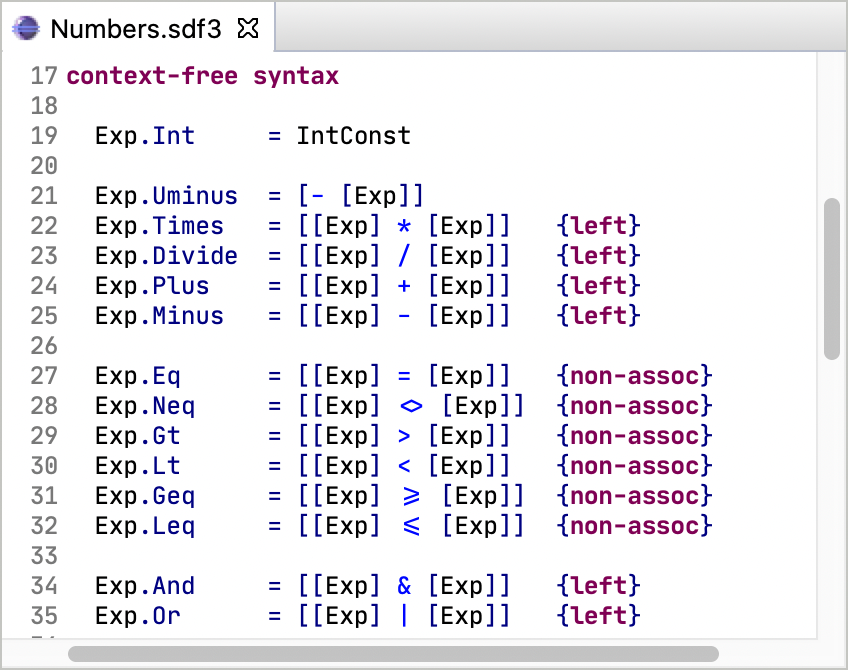
\includegraphics[width=0.8\linewidth]{img/syntax}
\end{figure}
\end{frame}

\begin{frame}[fragile]{Background: What is Spoofax?}
	\begin{figure}
		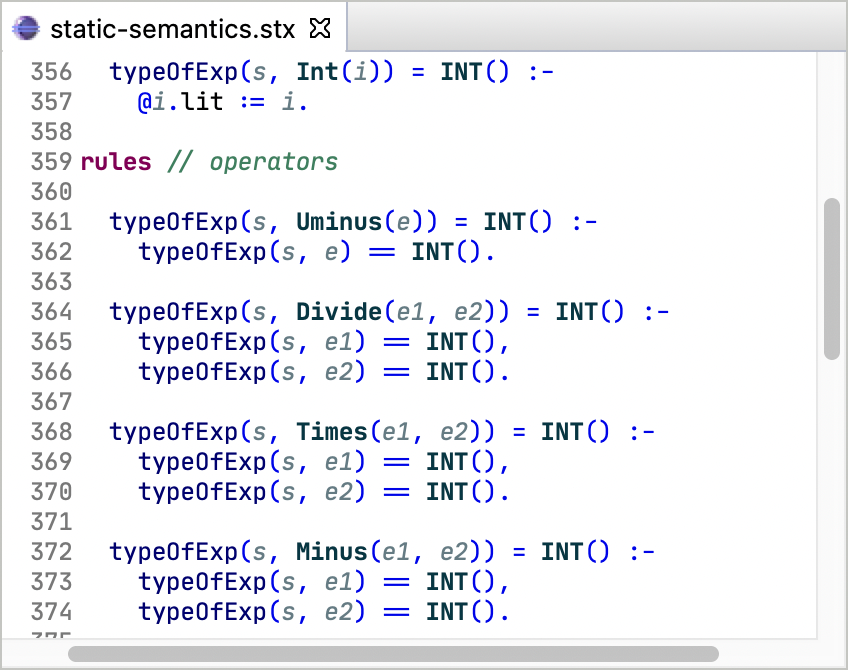
\includegraphics[width=0.8\linewidth]{img/semantics}
	\end{figure}
\end{frame}

\begin{frame}[fragile]{Background: What is Spoofax?}

\begin{exampleblock}{Example}
\begin{lstlisting}
let x = 5;
let y = x + 3;
return x + y;
\end{lstlisting}
\end{exampleblock}

\begin{figure}
	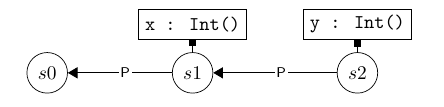
\includegraphics[width=0.7\linewidth]{img/screenshot005}
\end{figure}

% The logic I just explained would be written down in Statix
% Like: When you encounter a let, create a new scope...

\end{frame}

\begin{frame}[fragile]{Background: What is Spoofax?}
	\begin{figure}
		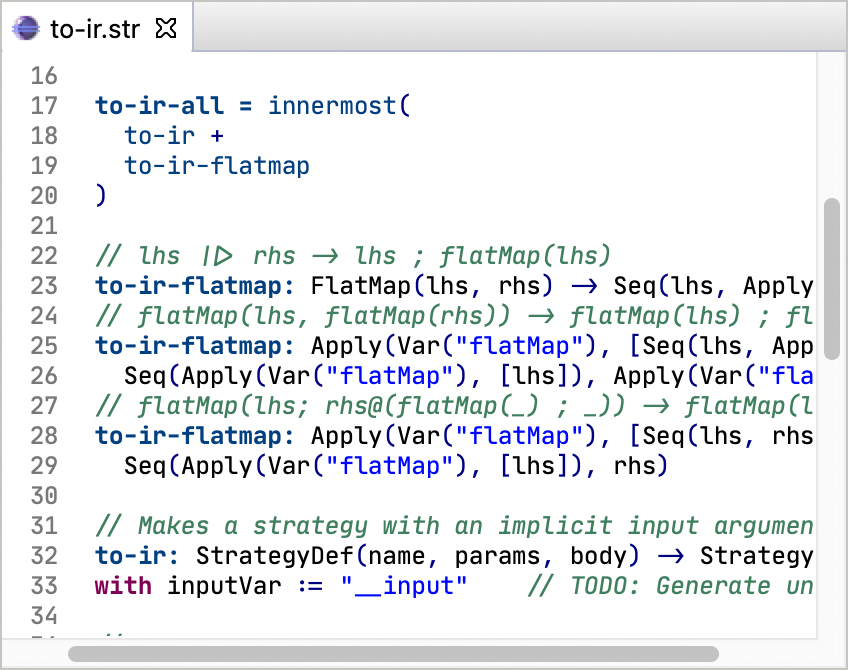
\includegraphics[width=0.8\linewidth]{img/transformation}
	\end{figure}
	% - used for interpreters (3+5=8) or compiler (a+b compiles to add instruction in x86)
	% - = DYNAMIC SEMANTICS
\end{frame}

\begin{frame}[fragile]{Background: What are Dependent Types?}
\begin{itemize}
	\item Types may depend on values!
	\begin{exampleblock}{Example}
		\texttt{concat : (A: Type) -> (n m : Nat) -> Vec A n -> Vec A m
			\\ \hspace*{48pt} -> Vec A (n + m)}
	\end{exampleblock}
% - n occurs insie a type `Vec`!
% - The type system enforces these lengths are always correct
% - Challenge: Type checking may require evaluating arbitrary terms to decide equality
\end{itemize}
\end{frame}

\begin{frame}[fragile]{Background: What are Dependent Types?}
	Why are dependent types useful?
	\begin{itemize}
		\item Proof Assistants: Agda, Lean, Coq, etc
	\end{itemize}
	
	% We're looking only at signatures
	\begin{exampleblock}{Sorted lists}
\texttt{sort : List t -> List t\\sort\_sorted : (v : List t) -> IsSorted (sort v)}
	\end{exampleblock}
\end{frame}

\begin{frame}[fragile]{Background: What are Dependent Types?}
	Type checking requires evaluation
	\begin{exampleblock}{Example 1}
		\texttt{let T: Type = if false then Int else Bool end;\\let b: T = true;}
	\end{exampleblock}
\end{frame}

\begin{frame}[fragile]{Research Question}
\large{How suitable is Statix for defining a dependently-typed language?}
\begin{itemize}
	\item Will it be easier than doing it in Haskell?
	\item Prior work: Defining System F\footnote{Hendrik van Antwerpen et al. Scopes as types.}
\end{itemize}

% Mention system f (polymorphic lambda calculus) being hard (scopes as types)
% Statix is turing complete, so it's going to be possible
% But is it going to be easier or harder than a general purpose language like haskell?
\end{frame}

\begin{frame}[fragile]{Why is this important?}
	\begin{block}{Spoofax perspective}
		Developing a language with a complex type system tests the boundaries of what Spoofax can do.
	\end{block}
	% - What can we improve about Statix?
	
	\begin{block}{Dependent Types perspective}
		Using a language workbench helps with rapid prototyping.
	\end{block}
	% - Try a new feature without having to implement in general purpose
	% - Spoofax provides an easy way to get a parser, type checker, etc
\end{frame}

\begin{frame}[fragile]{Primary Contribution: Calculus of Constructions in Statix}
	A lambda calculus with dependent types.
	
	\begin{block}{Syntax Definition}
		\begin{figure}
			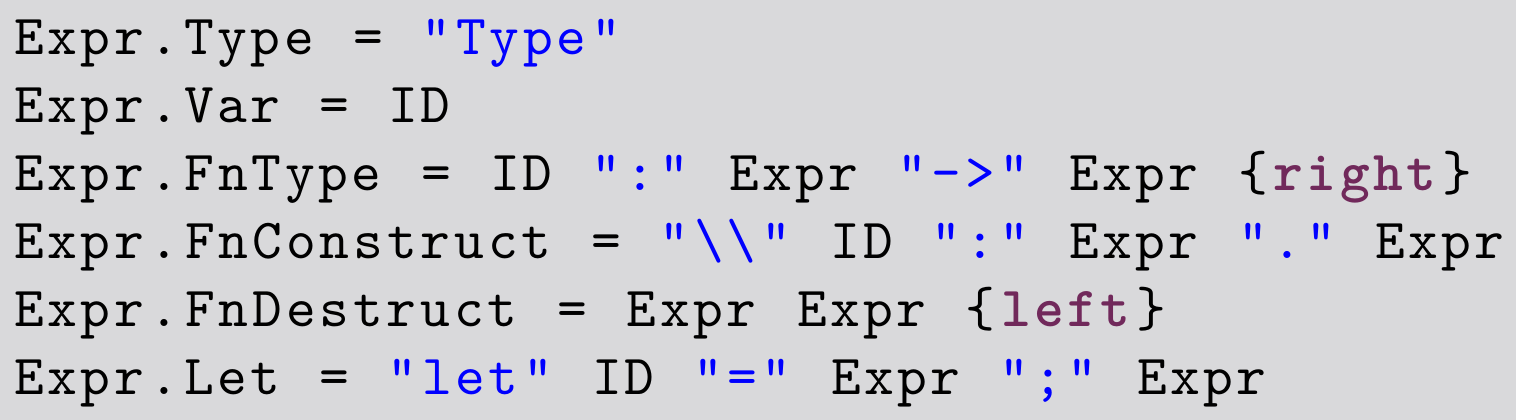
\includegraphics[width=0.7\linewidth]{img/screenshot006}
		\end{figure}
	\end{block}

	\begin{exampleblock}{Example}
		\texttt{let f = $\backslash$T: Type. $\backslash$x: T. x; \\
f (Type -> Type) ($\backslash$y: Type. y)
		}
	\end{exampleblock}

	% most simple dependently typed language: lambda calculus
	% what other languages use as a core
\end{frame}

\begin{frame}[fragile]{Type Checking}
	\begin{figure}
		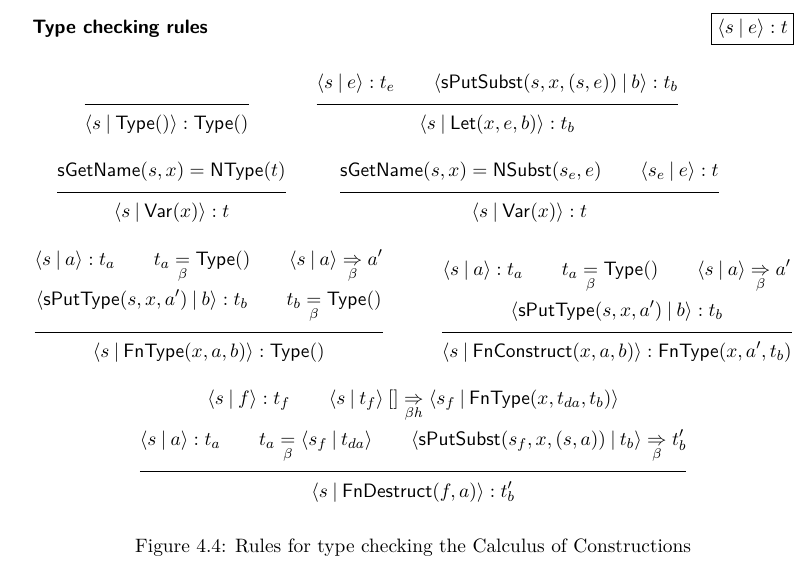
\includegraphics[width=0.9\linewidth]{img/screenshot007}
	\end{figure}
	% We define the language using inference rules
	% How can we express those rules in Statix?
\end{frame}

\begin{frame}[fragile]{Type Checking: From inference rules to Statix code}
	\begin{figure}
		\centering
		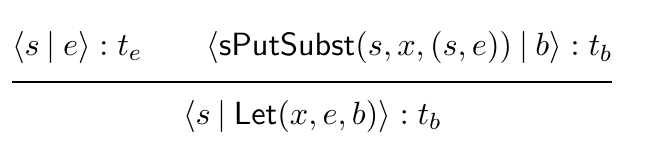
\includegraphics[width=0.8\linewidth]{img/screenshot004}
	\end{figure}
	
	\begin{block}{Signature of \emph{typeOfExpr}}
		\texttt{typeOfExpr : scope * Expr -> Expr}
	\end{block}
	
	\begin{exampleblock}{Equivalent Statix code} 
		\texttt{typeOfExpr (s, Let(x, e, b)) = bt :-\\
			\,\, typeOfExpr (s, e) == et, \\
			\,\, typeOfExpr (sPutSubst (s, x, (s, e)), b) == bt}
	\end{exampleblock}
\end{frame}

\begin{frame}[fragile]{Type Checking: Environments \& Context}
	\begin{exampleblock}{Example}
		\texttt{let T: Type = Bool;\\
			$\backslash$b: T. ???
		}
	\end{exampleblock}
	
	\begin{block}{What information is needed?}
		\begin{enumerate}
			\item T = Bool (Stored in Environment)
			\item b : T (Stored in Context)
		\end{enumerate}
	\end{block}
\end{frame}


\begin{frame}[fragile]{Type Checking: Environments \& Context}
	\begin{block}{How do we use scopes?}
		Scope graphs are used as a replacement for an environment and a context.
	\end{block}
	
	\begin{figure}
		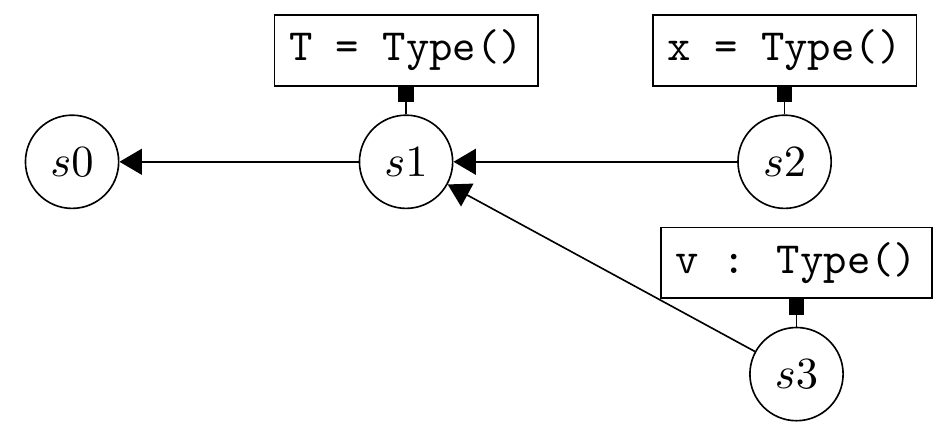
\includegraphics[width=0.7\linewidth]{screenshot005}
	\end{figure}
	
\end{frame}

\begin{frame}[fragile]{Type Checking: Requires Evaluation}
	\begin{exampleblock}{Example from earlier}
		\texttt{let T = if false then Int else Bool end;\\let b: T = true;}
	\end{exampleblock}
	\begin{block}{Evaluation relation} 
		\texttt{betaHeadReduce : scope * Expr -> scope * Expr} \\
		\texttt{betaReduce : scope * Expr -> Expr} \\
		\texttt{expectBetaEq : (scope * Expr) * (scope * Expr)}
	\end{block}
\end{frame}

\begin{frame}[fragile]{Type Checking: Requires Evaluation}
	\begin{figure}
		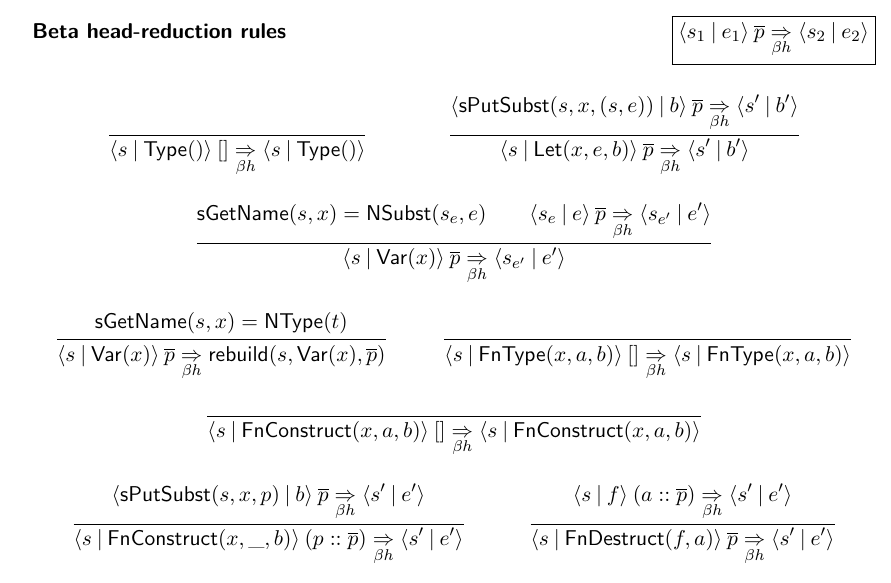
\includegraphics[width=0.9\linewidth]{screenshot001}
	\end{figure}
	
	% Talk about the fact that we're now defining evaluation in Statix
\end{frame}

\begin{frame}[fragile]{Type Checking: Variable Capturing}
	\begin{exampleblock}{What is the type of this expression?}
		\texttt{$\backslash$T : Type. $\backslash$T : T. T}
	\end{exampleblock}
\end{frame}

\begin{frame}[fragile]{Type Checking: Variable Capturing}
	\begin{exampleblock}{What is the type of this expression?}
		\texttt{$\backslash$T : Type. $\backslash$T : T. T}
	\end{exampleblock}
	
	\begin{block}{The type}
		\texttt{T : Type -> T : T -> T}
	\end{block}
	
	\begin{block}{Equivalent type under renaming: Not correct!}
		\texttt{T : Type -> x : T -> x}
	\end{block}
\end{frame}

\begin{frame}[fragile]{Type Checking: Variable Capturing}
	\begin{block}{Solutions}
		\begin{enumerate}
			\item De Bruijn indices
			\item Uniquifying names
			\item Capture-avoiding substitution
			\item \textbf{Using scopes to distinguish names}
		\end{enumerate}
	\end{block}
	
	\begin{block}{The type}
		\texttt{T : Type -> T : T -> T}
	\end{block}
	
	\begin{block}{The type (fixed)}
		\texttt{T : Type -> T : (T, s0) -> (T, s0)}
	\end{block}
\end{frame}



\begin{frame}[fragile]{Extra contributions}
	% Refer to thesis for this
Features
\begin{enumerate}
	\item Implemented Inference
	\item Implemented Inductive Data Types
	\item Implemented Universes
	\item Interpreter
	\item Compiler to Clojure
\end{enumerate}
Evaluation
\begin{enumerate}
	\item Comparison with implementation in Haskell
	\item Comparison with implementation in LambdaPi
	\item Evaluation of Spoofax
\end{enumerate}
\end{frame}

\begin{frame}{On Extensibility}
	\begin{block}{How to extend the language}
		\begin{enumerate}
			\item Define parsing rules
			\item Create a new .stx file
			\item Define the relations: \texttt{typeOfExpr, betaReduceHead, expectBetaEq and betaReduce}
		\end{enumerate}
	\end{block}
\end{frame}

\begin{frame}{Comparison with Haskell}
	\begin{block}{Type checking}
		\texttt{data EnvEntry = NType Expr | NSubst (Env, Expr)
			\\type Env = [EnvEntry]
			\\tc :: Env -> Expr -> Either String Expr}
	\end{block}

	\begin{block}{Differences}
		\begin{itemize}
			\item Distribution of definitions over files
			\item De Bruijn Indices vs Names
			\item Inference built-in to Statix
		\end{itemize}
	\end{block}
\end{frame}

\begin{frame}{Term Inference}
	\begin{example}\texttt{let id = ($\backslash$T : Type. $\backslash$x: T. x);
	\\id \_ true}
	\end{example}
	\begin{block}{How it works}
		\begin{itemize}
			\item When \texttt{expectBetaEq(e1, e2)} and \texttt{e1} or \texttt{e2} is free, infer!
			\item But in Statix we can't query whether variables are free.
			\item Solution: Wrap each free constructor in \texttt{Infer}.
		\end{itemize}
	\end{block}
\end{frame}

\begin{frame}{Term Inference: Equational Unification}
	\begin{itemize}
		\item We can declare two terms to be equal if they satisfy a certain relation (such as beta equality)
		\item We do this using \emph{reduction rules}, such as:
		\begin{exampleblock}{Example of a rewrite rule}
			($\backslash$ x : T. b) a => b[x := a]
		\end{exampleblock}
		\item Comparison with LambdaPi
	\end{itemize}
\end{frame}

\begin{frame}[fragile]{Conclusions}
	Spoofax is a great tool for developing dependently typed languages!
	\begin{itemize}
		\item We can use scopes to represent environments and contexts
		\item Statix can still use improvements
		% - Higher order 
	\end{itemize}
	
	%- using scopes as env+context  
	%- statix enforces syntactic uniqueness of metavariable solutions but dependently typed languages use a weaker notion of equality 
	%- full thesis coming soonTM
\end{frame}

% block
% exampleblock
% alertblock

\end{document}

